\section{Organisation}
\label{cha:Organisation}
In diesem Abschnitt wird das Projektmanagement des Teams beschrieben, das zum erfolgreichen Abschluss des Projektes beigetragen hat. Bei einem Team mit fünf Personen ist es wichtig Maßnahmen zur Dateiverwaltung und Organisation zu treffen, um eine gute Zusammenarbeit zu gewährleisten.

\subsection{Gruppentreffen und Organisation}
\label{sec:gruppentreffenundorganisation}
Im Folgenden werden die Gruppentreffen und das Team an sich beschrieben.
\paragraph{Gruppentreffen}
Bei dem ersten Teamtreffen wurde entschieden welche Versionsverwaltung und Organisationsplattform verwendet wird, diese wurden zusammen eingerichtet.

Im zwei Wochen Takt traf sich vorzugsweise das gesamte Team mit einem Betreuer des Projektes. Mit ihm wurde der aktuelle Stand des Projektes besprochen und gegebenenfalls Probleme im Team dargelegt. Diese Treffen waren organisatorischen Zwecken gewidmet, es wurden keine Fragen direkt zur Implementierung geklärt. Als das Projekt grundlegend funktionierte, wurden Anregungen zur Erweiterung der Aufgabenstellung gegeben. 

Zur Besprechung von Regelungs- und Implementierungsfragen, gab es annähernd jede zweite Woche ein Regelungstechniktreffen, bei dem sich zwei Teammitglieder jeder Gruppe einfanden. Die Teilnehmer tauschten sich untereinander über den Stand der jeweiligen Gruppen aus und diskutierten verschiedene Fragen. Für weitere Fragen und Anregungen stand dort ein Betreuer der Regelungstechnik zur Verfügung.

Zusätzlich zu den Beratungsgesprächen wurden wöchentliche Treffen mit allen Gruppenmitgliedern festgelegt. Jeder berichtete von seinem Vorgehen der vergangenen Woche, so dass alle im Team den Überblick über den aktuellen Stand des Projektes hatten. Daraufhin wurden Ideen und Anregungen zusammengetragen und die Planung für die nächste Woche erarbeitet. Mit Hilfe der im \autoref{sec:aufgabenverwaltung} noch erwähnten Organisationsplattform Trello wurden die Aufgaben erfasst und den interessierten Gruppenmitgliedern zugeordnet. 


\paragraph{Team}

Die Zeitplanung wurde dynamisch gehalten, da es schwer einschätzbar ist, wie viel Zeit eine einzelne Aufgabe in Anspruch nehmen wird. Erfahrungen aus anderen Projekten haben gezeigt, dass dieses Vorgehen sinnvoll ist. Um genügend Zeit für die Optimierung und Dokumentation einzuplanen und gegebenenfalls einen ausreichenden Zeitpuffer zur Verfügung zu haben, wurde als Ziel festgelegt, dass nach vier von fünf Monaten der Projektzeit eine funktionierende Version vorhanden sein soll. Jede Woche wurde bei dem Gruppentreffen festgelegt, wer sich welcher neuen Aufgabe annimmt und es wurde erneut abgeschätzt, wie viel Zeit eine angefangene Aufgabe noch beanspruchen wird.


Nachdem sich alle in die Dokumentation eingelesen hatten, wurden erste Grundlagen zusammen erarbeitet, damit jeder ein Grundwissen über das Modellauto hatte. Es bildeten sich Aufgabengruppen für Organisation, Regelung und Bildverarbeitung, diese wurden weitestgehend parallel behandelt. Die Verantwortung für diese Teilgruppen wurde auf die Mitwirkenden aufgeteilt. Jedes Gruppenmitglied konnte bei jeder Aufgabengruppe helfen, allerdings ist es wichtig Verantwortliche festzulegen, um den Überblick zu bewahren und zielführend zu agieren. Als die Tests der Bildverarbeitung und Regelung die aufgestellten Bedingungen erfüllten, wurden diese Aufgabenbereiche zusammengeschlossen und es wurde dadurch das Fahren durch den Rundkurs erlangt. Neben der Optimierung des Rundkurses wandte sich eine Subgruppe dem zweiten Thema, Hinderniserkennung mit Spurwechsel, zu.

Es gab viele Aufgaben, die direkt am Fahrzeug getestet werden mussten. Da das gleichzeitige Testen mehrerer Aufgaben meist nicht möglich war, wurden die anderen Teammitglieder beim Zusammenkommen über die Aufgabenverteilung hinaus unterstützt. Jeder teilte sich seine Zeit jede Woche selbst ein und kommunizierte, welche Aufgabe wann bearbeitet wird, damit Interessengruppen zusammenfinden konnten. 


\subsection{Aufgabenverwaltung}
\label{sec:aufgabenverwaltung}
Für die Planung der Aufgaben wurde die web-basierte Projektmanagementsoftware Trello\footnote{https://trello.com/} verwendet. Durch Visualisierung im Karteikastensystem wurde der Überblick über die bevorstehenden Aufgaben und die dazugehörenden Verantwortlichen bewahrt. Zusätzlich gab es Farblabel, um die zusammengehörenden Aufgaben visuell zu markieren. Das Board wurde in Kategorien, wie \textit{ToDo, Im Gange, Testen, Fertig und Zurückgestellt/Gescheitert}, aufgeteilt. Die einzelnen Aufgaben wurden je nach Aufgabenstatus in die zutreffende Kategorie verschoben. 

\begin{figure}[h]
	\centering
	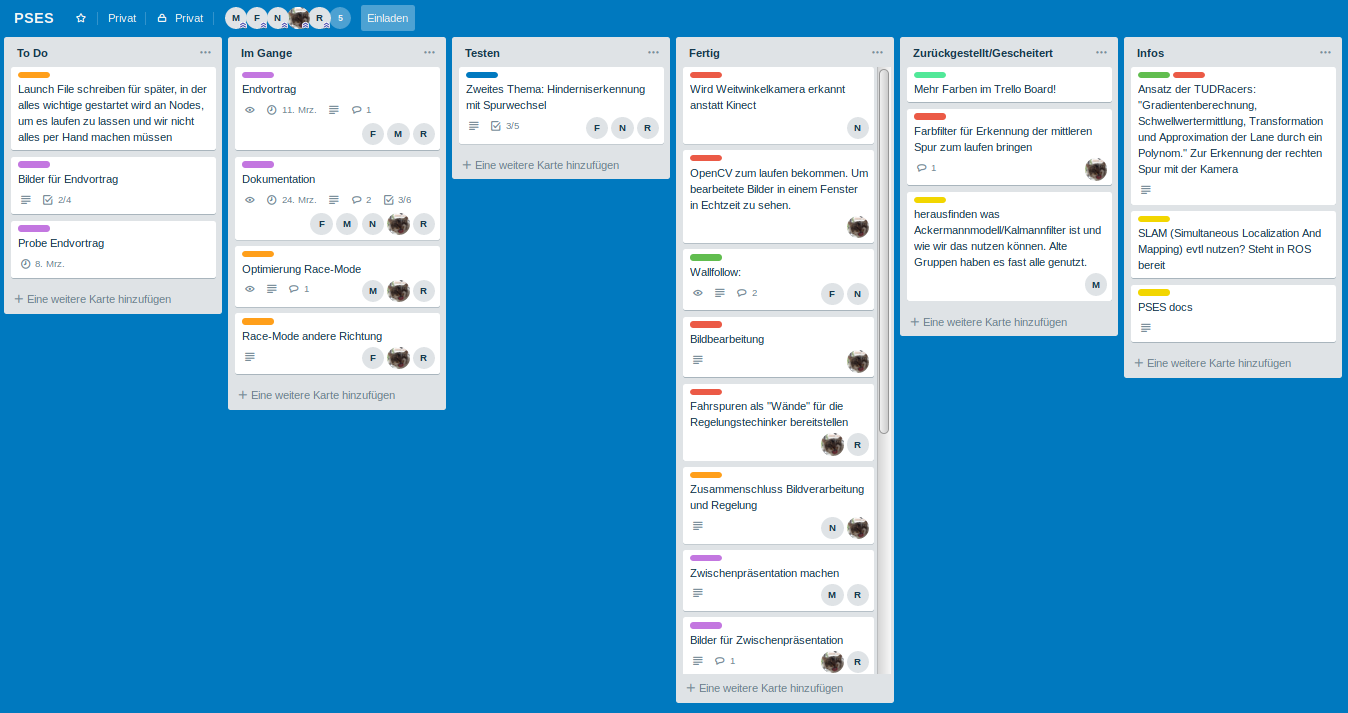
\includegraphics[width=0.9\textwidth]{images/Trello.png}
	\caption{Trello-Board von Team AUDO zum Projektstand: Optimierung der einzelnen Fahrmodi}
	\label{abb:trello-board}
\end{figure}


\subsection{Versionsverwaltung}
\label{sec:versionsverwaltung}
Angesichts guter Erfahrungen stand schnell fest, dass GitHub\footnote{https://github.com/} als Versionsverwaltung verwendet wird. Die meisten Teammitglieder verfügten bereits über Kenntnisse mit GitHub und mussten sich nicht in neue Verwaltungsstrukturen einarbeiten. Der Vorteil von Versionsverwaltungen ist, dass alte Programmierzustände gesichert sind und man diese wieder herstellen kann. Durch die Versionierung des Quellcodes mit GitHub wurde das fehlerfreie Programmieren im Team sichergestellt. Ohne Verwaltung des Quellcodes ist es fehleranfällig  mit mehreren Leuten an dem gleichen Programmiercode zu arbeiten.
Über GitHub wurden zusätzlich zu dem Quellcode die Vortragsfolien und die Dokumentation verwaltet.